\chapter{Методы}
С точки зрения машинного обучения и нейронных сетей есть множество важных аспектов,
помимо точности. В контексте физически-информированных нейронных сетей речь пойдет
об оптимизации архитектуры нейронной сети для ускорения обучения, увеличения точности
для оценки компонент скоростей или давления \cite{Tommaso2024pinn}.

Нейронные сети весьма непредсказуемы при обучении, особенно в случае отсутствия
обучающих и тестовых данных. Для понимания работы нейронных сетей в таком режиме
следует изучить влияние количества нейронов, активационной функции, количества слоев,
Dropout'ов, а также обратить внимание на функции активации, которые определяют,
как нейрон будет реагировать на входные данные, что может существенно влиять на способность
сети обучаться сложным функциям и обобщать полученные данные.
\section{Постановка задачи}
В основе исследуемых задач будем использовать уравнения Навье-Стокса по следующим
причинам:
\begin{enumerate}
    \item Данные уравнения используют частные производные первого и второго порядка
    \item Подразумевается система трех уравнений для двумерной задачи
    \item Наличие двух входных и трех выходных переменных для двумерной задачи
\end{enumerate}
Такой подход позволит рассмотреть физически-информированные нейронные сети на сложных,
с точки зрения модели, задачах, тем самым изучив поведение модели в нетривиальных случаях.

Для анализа будут рассмотрены течение Куэтта и течение жидкости в канале
\subsection{Течение Куэтта}
\begin{figure}[ht]
    \caption{Постановка задачи течения Куэтта}
    \label{fig:couette_flow}
    \centering
    \begin{tikzpicture}[scale=1.5]

        % Оси координат
        \draw[->] (0,0) -- (7,0) node[below] {$x$};
        \draw[->] (0,0) -- (0,3) node[left] {$y$};
    
        % Пластины
        \draw[thick] (0,0.5) -- (6.5,0.5) node[midway, below] {Нижняя пластина ($u=0$)};
        \draw[thick] (0,2.5) -- (6.5,2.5) node[midway, above] {Верхняя пластина ($u=U_0$)};
    
        % Расстояние между пластинами
        \draw[decorate, decoration={brace, amplitude=5pt, mirror}] (6.7,0.5) -- (6.7,2.5) 
            node[midway, right=5pt] {$h$};
    
        % Течение Куэтта (линейный профиль скорости)
        \foreach \y in {0.6,0.8,...,2.4} {
            \pgfmathsetmacro{\arrowlength}{2*(\y-0.5)/2} % Вычисляем длину стрелки
            \draw[blue, ->] (0,\y) -- (0+\arrowlength,\y); % Рисуем стрелку
        }
    
        % Подписи
        \node at (3,1.5) {$\vec{u}(y) = U_0 \frac{y}{h}$};
        
    \end{tikzpicture}
\end{figure}
\begin{figure}[ht]
    \caption{}
    \label{points}
    \centering
    \resizebox{0.8\columnwidth}{!}{
        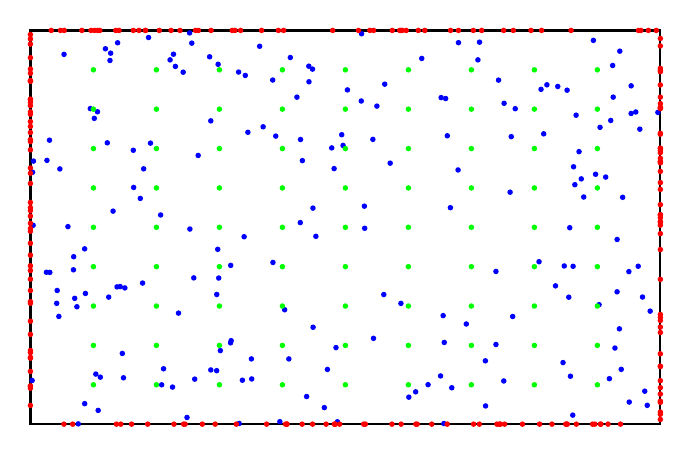
\begin{tikzpicture}
            % Прямоугольник  (размеры 8x5)
            \draw[thick] (-4,-2.5) rectangle (4,2.5);

            % Случайные точки внутри прямоугольника
            \foreach \i in {1,...,200} {
                \fill[blue] (rand*4, rand*2.5) circle (1pt);
            }

            % Случайные точки на гранях прямоугольника
            \foreach \i in {1,...,50} {
                % Нижняя грань
                \fill[red] (rand*4, -2.5) circle (1pt);
                % Верхняя грань
                \fill[red] (rand*4, 2.5) circle (1pt);
                % Левая грань
                \fill[red] (-4, rand*2.5) circle (1pt);
                % Правая грань
                \fill[red] (4, rand*2.5) circle (1pt);
            }

            \foreach \i in {-4,...,4} {
                \foreach \j in {-4,...,4} {
                    \fill[green] (4 * \i / 5, 2.5  * \j / 5) circle (1pt);
                }
            }
        \end{tikzpicture}
        }
    \end{figure}
Течение Куэтта представляет из себя двумерный плоский канал шириной $l$, одна из стенок которого 
движется со скоростью $u_0$. Данная задача имеет аналитическое решение:
\begin{equation}
    \begin{cases}
        u = u_0 * y / l \\
        v = 0
    \end{cases}
\end{equation}
где $y$ --- расстояние от неподвижной стенки.
Используя данное аналитическое решение можно валидировать результаты нейронной сети и
исследовать влияение наличия правильного решения в процессе обучения нейронной сети на
резульаты.
\subsection{Течение жидкости в канале}
Для усложнения задачи возьмем канал, отличный от плоского. \textcolor{red}{На занятиях
по дисциплине "Компьютерное моделирование прикладных физических задач" мы решали подобную
задачу посредством традиционных численных методов???}. Канал представляет из себя (рисунок).
\include{images/tikz/channel_flow.tex}
Возьмем ранее упомянутое численное решение для оценки качества результата нейронной сети и
последующего внедрения данных точного решения в процесс обучения.


% MFN-PINN,  MLP-PINN

Каждый нейрон в нейронной сети использует функцию активации для преобразования взвешенной
суммы своих входных сигналов в выходной сигнал. Эта функция вносит нелинейность в модель,
что необходимо для обучения сложных зависимостей.

Формула, описывающая этот процесс, выглядит следующим образом:

$$y = f(\sum_{i=1}^{n} w_i x_i + b)$$

где $x_i$ — $i$-й входной сигнал нейрона, $w_i$ — вес, связанный с $i$-м входным сигналом, $b$
— смещение нейрона, $f(\cdot)$ — функция активации, $y$ — выходной сигнал нейрона.

Для эффективного использования в PINNs функции активации должны удовлетворять следующим
критериям \cite{0d752c79fb816703274a3d37f85a85689a2a9405}:
\begin{itemize}
    \item функции активации должны быть гладкими и
    непрерывно дифференцируемыми, чтобы обрабатывать функции потерь, которые включают
    производные высших порядков.
    \item функции активации должны допускать неограниченные
    выходные значения, в отличие от функций $tanh$ и $sin$, которые ограничены между $-1$ и $1$.
    \item функции активации должны избегать насыщения, чтобы предотвратить
    исчезновение градиентов, что может затруднить обучение.
    \item в некоторых случаях желательно иметь контролируемое насыщение за пределами определённого
    диапазона, чтобы улучшить способность модели представлять сложные физические сигналы.
\end{itemize}


\subsection{ReLU}
\begin{figure}[ht]
    \caption{Функции активации на основе Swish}
    \label{fig:act_func_graph}
    \centering
    \begin{tikzpicture}
        \begin{axis}[
            width=14cm, height=10cm,
            grid=both,
            axis y line=middle, axis x line=middle,
            ymin=-1.2, ymax=1.2,
            xmin=-5, xmax=5,
            samples=201,
            legend style={at={(0.5,-0.1)},anchor=north,legend columns=2},
            legend cell align={left},
            title={Активационные функции}
        ]
        
        % Пороговая функция (Heaviside, Step)
        \addplot[thick, blue, domain=-5:5] {x >= 0 ? 1 : 0};
        \addlegendentry{Пороговая (Heaviside)}
        
        % Сигмоида (Logistic Sigmoid)
        \addplot[thick, red, domain=-5:5] {1/(1+exp(-x))};
        \addlegendentry{Сигмоида (Logistic)}
        
        % Гиперболический тангенс (tanh)
        \addplot[thick, green!70!black, domain=-5:5] {tanh(x)};
        \addlegendentry{Гиперб. тангенс (tanh)}
        
        % ReLU
        \addplot[thick, orange, domain=-5:5] {x > 0 ? x : 0};
        \addlegendentry{ReLU}
        
        % Сигмоида сдвинутая (Bipolar Sigmoid)
        \addplot[thick, magenta, domain=-5:5] {(1 - exp(-x))/(1 + exp(-x))};
        \addlegendentry{Сигмоида сдвинутая (Bipolar)}
        
        % Гауссова функция
        \addplot[thick, cyan, domain=-5:5] {exp(-x^2)};
        \addlegendentry{Гауссова функция}
        
        \end{axis}
    \end{tikzpicture}
    
\end{figure}
\begin{figure}[ht]
    \caption{Функции активации на основе REAct}
    \label{fig:react_func_graph}
    \centering
    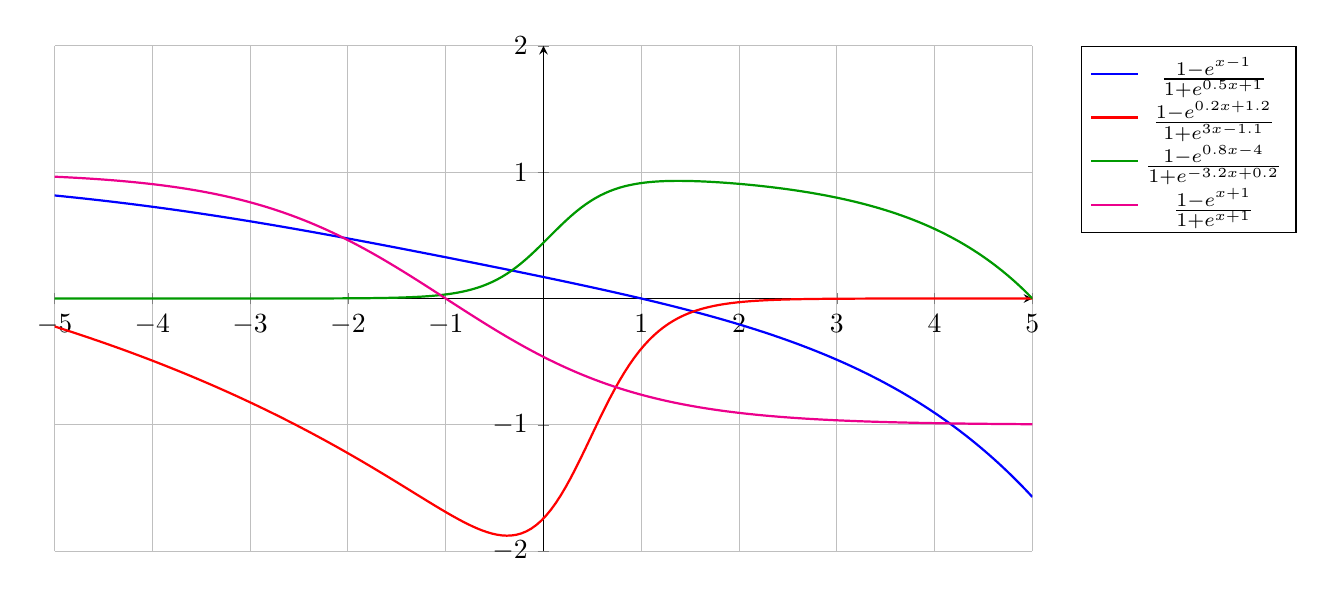
\begin{tikzpicture}
        \begin{axis}[
            width=14cm,
            height=8cm,
            xmin=-5, xmax=5,
            ymin=-2, ymax=2,
            axis lines=middle,
            grid=both,
            legend style={at={(1.05,1)},anchor=north west}
        ]
        % 1. [1, -1, 0.5, 1]
        \addplot[
            domain=-5:5, 
            samples=200, 
            thick, 
            blue
        ]
        {(1 - exp(1*x - 1)) / (1 + exp(0.5*x + 1))};
        \addlegendentry{$\frac{1 - e^{x - 1}}{1 + e^{0.5x + 1}}$}
        
        % 2. [0.2, 1.2, 3, -1.1]
        \addplot[
            domain=-5:5, 
            samples=200, 
            thick, 
            red
        ]
        {(1 - exp(0.2*x + 1.2)) / (1 + exp(3*x - 1.1))};
        \addlegendentry{$\frac{1 - e^{0.2x + 1.2}}{1 + e^{3x - 1.1}}$}
        
        % 3. [0.8, -4, -3.2, 0.2]
        \addplot[
            domain=-5:5, 
            samples=200, 
            thick, 
            green!60!black
        ]
        {(1 - exp(0.8*x - 4)) / (1 + exp(-3.2*x + 0.2))};
        \addlegendentry{$\frac{1 - e^{0.8x - 4}}{1 + e^{-3.2x + 0.2}}$}
        
        % 4. [1, 1, 1, 1]
        \addplot[
            domain=-5:5, 
            samples=200, 
            thick, 
            magenta
        ]
        {(1 - exp(1*x + 1)) / (1 + exp(1*x + 1))};
        \addlegendentry{$\frac{1 - e^{x + 1}}{1 + e^{x + 1}}$}
        
        \end{axis}
    \end{tikzpicture}
    
\end{figure}
\begin{figure}[ht]
    \caption{Функции активации на основе REAct}
    \label{act_func_graph}
    \centering
    \begin{tikzpicture}
        \begin{axis}[
            width=16cm,
            height=10cm,
            xmin=-4, xmax=4,
            ymin=-3, ymax=8,
            axis lines=middle,
            grid=both,
            legend style={at={(1.05,1)},anchor=north west, font=\footnotesize},
            cycle list name=color list,
            samples=200
        ]
        
        % Функция swish(x) = x * sigmoid(x)
        \pgfmathdeclarefunction{swish}{1}{
          \pgfmathparse{#1/(1+exp(-#1))}
        }
        
        % Функция softplus(x) = ln(1 + exp(x))
        \pgfmathdeclarefunction{softplus}{1}{
          \pgfmathparse{ln(1 + exp(#1))}
        }
        
        % Перебор всех комбинаций (a, b, c, d)
        \foreach \a/\b/\c/\d in {0/0/0/0, 0/0/0/1, 0/0/1/0, 0/0/1/1,
                                 0/1/0/0, 0/1/0/1, 0/1/1/0, 0/1/1/1,
                                 1/0/0/0, 1/0/0/1, 1/0/1/0, 1/0/1/1,
                                 1/1/0/0, 1/1/0/1, 1/1/1/0, 1/1/1/1}
        {
            \addplot+[thick] 
            ({x},
             {sin(deg(x)) 
              + (\a == 1 ? tanh(x) : 0)
              + (\b == 1 ? swish(x) : 0)
              + (\c == 1 ? 1/(1 + x^2) : 1)
              + (\d == 1 ? softplus(x) : 0)
             });
            % \addlegendentry{$a=\a,\,b=\b,\,c=\c,\,d=\d$}
        }
        
        \end{axis}
    \end{tikzpicture}
    
\end{figure}
\begin{figure}[ht]
    \caption{Структура PINN с использованием функции активации Adaptive Blending Unit\cite{a104fe01d341f235fd80ea98d6a8f35b8110df1d}}
    \label{pinn_structure}
    \centering
    \resizebox{0.8\columnwidth}{!}{
        \begin{tikzpicture}[]
            % Цвета
            \definecolor{inputcolor}{RGB}{173,216,230}
            \definecolor{weightcolor}{RGB}{255,228,181}
            \definecolor{sumcolor}{RGB}{255,182,193}
            \definecolor{actcolor}{RGB}{144,238,144}
            \definecolor{outputcolor}{RGB}{255,255,224}

            % Входы
            \node[draw, circle, fill=inputcolor] (x1) {$x_1$};
            \node[draw, circle, fill=inputcolor, below=0.9cm of x1] (x2) {$x_2$};
            \node[below=0.5cm of x2] (dots) {$\vdots$};
            \node[draw, circle, fill=inputcolor, below=0.5cm of dots] (xn) {$x_n$};

            % Веса
            \node[draw, circle, fill=weightcolor, right=1.2cm of x1] (w1) {$w_{j1}$};
            \node[draw, circle, fill=weightcolor, right=1.2cm of x2] (w2) {$w_{j2}$};
            \node[draw, circle, fill=weightcolor, right=1.2cm of xn] (wn) {$w_{jn}$};

            % Сумматор
            \node[draw, circle, fill=sumcolor, right=2.2cm of w2, minimum size=1.2cm] (sum) {$\sum$};

            % Функция активации
            \node[draw, rectangle, fill=actcolor, right=2.2cm of sum, minimum width=1.2cm, minimum height=1.2cm] (phi) {$\varphi$};

            % Выход
            \node[draw, circle, fill=outputcolor, right=2.2cm of phi] (out) {$o_j$};

            % Стрелки входов к весам
            \draw[->] (x1) -- (w1);
            \draw[->] (x2) -- (w2);
            \draw[->] (xn) -- (wn);

            % Стрелки весов к сумматору
            \draw[->] (w1) -- (sum);
            \draw[->] (w2) -- (sum);
            \draw[->] (wn) -- (sum);

            % Стрелка из сумматора в функцию активации
            \draw[->] (sum) -- (phi);

            % Стрелка из функции активации в выход
            \draw[->] (phi) -- (out);

            % Смещение (порог)
            \node[above=0.5cm of phi] (theta) {$\theta_j$};
            \draw[->, dashed] (theta) -- (phi);

            % Подписи
            \node[above=0.25cm of x1] {Входы};
            \node[above=0.25cm of w1] {Веса};
            \node[above=0.25cm of sum] {Сумма входов};
            \node[below=0.25cm of phi] {Функция активации};
            \node[above=0.25cm of out] {Выход};


        \end{tikzpicture}       
    }
\end{figure}
ReLU (Rectified Linear Unit) — это функция активации, которая возвращает входное значение,
если оно положительное, и 0, если оно отрицательное \eqref{relu}. Это одна из самых популярных 
функций активации в нейронных сетях, благодаря своей простоте и эффективности. 
\begin{equation}
    \text{ReLU}(x) = \max(0, x)
    \label{relu}
\end{equation}
В контексте физически информированных нейронных сетей данная функция не эффективна в силу
разрава при $x = 0$ и производной, равной $1$ при положительных значениях $x$, что создает
проблемы при обратном распространении ошибки.

\subsection{SiLU}
SiLU (Sigmoid Linear Unit), также известная как $\text{Swish-}1$ \eqref{silu}, является
гладкой немонотонной функцией активации, используемой в нейронных сетях.
\begin{equation}
    \text{SiLU}(x) = x \cdot \sigma(x) \label{silu}
\end{equation}
Эта функция удобна своей гладкостью и способностью улучшать производительность глубоких
моделей машинного обучения по сравнению с функциями активации, такими как ReLU.
\subsection{Swish}
Swish является гладкой и немонотонной функцией, аналогично SiLU, но имеет дополнительный
параметр $\beta$, который может быть настроен или зафиксирован \eqref{swish}.
\begin{equation}
    \label{swish}
    swish_\beta(x) = \frac{x}{1 + e^{-\beta x}}
\end{equation}
В целом Swish является заменой всех предыдущих функций:
\begin{itemize}
    \item При $\text{swish}_1(x) = \text{SiLU}(x)$
    \item При $\text{swish}\inf(x) = \text{ReLU}(x)$
\end{itemize}

GELU (Gaussian Error Linear Unit) и
SILU (Sigmoid Linear Unit), а также стандартные ReLU (Rectified Linear Unit), Sigmoid
и Tanh. Помимо обычных функций активаций есть адаптивные, которые подразумевают подбор
специфичных коэфициентов в процессе обучения нейронной сети для улучшения "понимания"
физической составляющей искомой задачи. К таким функциям относятся функции ABU
(Adaptive Blending Unit) и REAct (Rational Exponential Activation)

